\documentclass[twoside]{article}
\usepackage[utf8]{inputenc}
\usepackage[ngerman]{babel}
\usepackage{libertine}
\usepackage[a4paper]{geometry}
\usepackage{parskip}
\usepackage{blindtext}
\usepackage{amsmath, amsthm, amssymb, commath, mathtools}
\usepackage{nicefrac}
\usepackage{booktabs}
\usepackage{tabularx}
\usepackage{enumitem}
\usepackage{graphicx}
\usepackage{minted}
\usepackage{appendix}
\usepackage{icomma}
\usepackage[separate-uncertainty=true]{siunitx}
\sisetup{locale = DE}

\usepackage{csquotes}
\MakeOuterQuote{"}
\renewcommand{\ttdefault}{cmtt}

\usepackage{hyperref}
\hypersetup{
	pdftitle={P1 -- STV Auswertung},
	pdfauthor={Yudong Sun, Andreas Artz},
	bookmarksnumbered=true,
	bookmarksopen=true,
	bookmarksopenlevel=2,
	pdfstartview=Fit,
	pdfpagemode=UseOutlines,
	colorlinks=true,
	linkcolor=black,
	filecolor=magenta,      
	urlcolor=blue
}
\urlstyle{same}

\title{STV -- Statistische Verteilung \\ Auswertung \\Nachbesserung}
\author{Yudong Sun, Andreas Artz \\ Gruppe F2}

\newcommand{\versuch}[0]{STV}

\usepackage{fancyhdr}
 
\pagestyle{fancy}
\fancyhf{}
\fancyhead[RO]{Yudong Sun, Andreas Artz}
\fancyhead[LO]{Auswertung -- \versuch}
\fancyhead[LE]{Yudong Sun, Andreas Artz}
\fancyhead[RE]{Auswertung -- \versuch}
\cfoot{\thepage}

\begin{document}

\maketitle

\section*{Teilversuch 1: Generierung einer Binomialverteilung mit dem Galton-Brett}

    \subsection*{Annahme: Die Verteilung der Kugeln ist bekannt}
        Bei jeder Weggabelung kann die Kugel entweder links oder rechts fallen. Damit die Kugel in den 0. Kanal fällt muss sie bei jeder Weggabelung im Galton-Brett nach links fallen, also insgesamt 10 mal. 
        \begin{align*}
            p(\text{Eine Kugel in Kanal 0}) &=\binom{10}{0} \times \frac{1}{2}^{10} \times \frac{1}{2}^0 \\
            &= \frac{1}{2^{10}} = \SI{0.0977}{}\% 
        \end{align*}
        Damit die Kugel in den 5. Kanal, der genau in der Mitte liegt, fällt, muss sie bei den Weggabelungen insgesamt 5 mal nach links und 5 mal nach rechts fallen. Die Reihenfolge ist dabei egal.
        \begin{align*}
            p(\text{Eine Kugel in Kanal 5}) &=\binom{10}{5} \times \frac{1}{2}^{5} \times \frac{1}{2}^{5} \\
            &= \SI{24.6}{}\% 
        \end{align*}
        
    \pagebreak
    \subsection*{Annahme: Die Verteilung der Kugeln ist unbekannt}
    
        \begin{figure}[!ht]
            \centering
            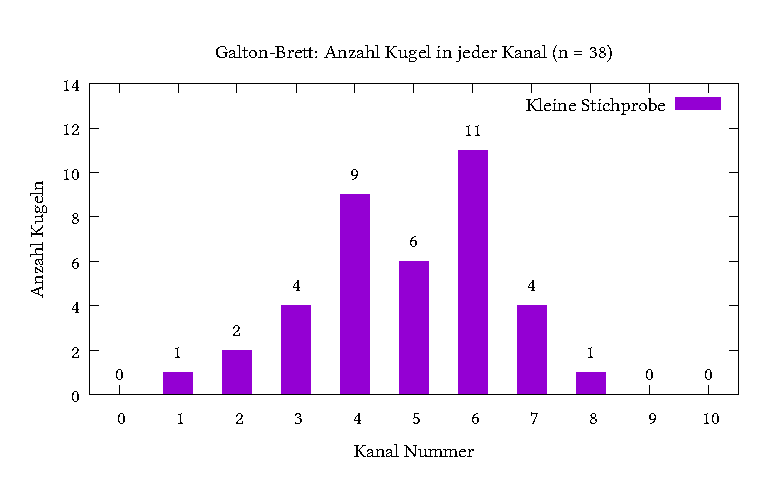
\includegraphics{kleine.eps}
            \caption{Histogramm der kleinen Statistik}
            \label{fig:kleine_histo}
        \end{figure}
        
        Die Mittelwert und Standardabweichung wird mithilfe eines Python-Skripts berechnet (Siehe Appendix \ref{appdx:codes}):
         \begin{center}
            \begin{tabular}{l l}
                \toprule
                Mittelwert & $4,8684$ \\
                Standardabweichung & $1,5968$ \\
                \bottomrule
            \end{tabular}
        \end{center}
        
         Man kann vom Histogramm nicht auf eine Binomialverteilung schließen. Zumindest ist das Histogramm nicht symmetrisch, und das Maximum ist nicht beim Mittelwert.
        
    \subsection*{Diskussion}
        Die Häufigkeits\-verteilungen sollten sich mit wachsender Stichprobengröße der Wahrscheinlichkeitsfunktion der Binomial\-verteilung annähern. Das Ergebnis zeigt dies, da die Verteilung der großen Statistik deutlich symmetrischer ist als die der mittleren Statistik. Zudem ist der Mittelwert der großen Statistik näher am Erwartungswert.

        Mit $N = 10$ und $p = \nicefrac{1}{2}$ lässt sich die theoretische Erwartungswert und Standardabweichung $\sigma$ einer binomischen Verteilung wie folgt berechnen:
        \begin{align}
            E(x) &= Np = 10 \times \frac{1}{2} = 5 \\
            \sigma &= \sqrt{Np(1-p)} = \sqrt{10\left(\frac{1}{2}\right)\left(1-\frac{1}{2}\right)} = \SI{1.581}{}
        \end{align}
        Die empirische Mittelwert und Standardabweichung liegen trotz des Histogrammes nahe an die theoretischen Werten. 

        \pagebreak
        \subsubsection*{Diskussion der Histogramme der mittleren und großen Statistik}
        \begin{center}
            \begin{tabular}{l | rrr}
                \toprule
                Stichprobe & $\bar{x}$ & $s$\\
                \midrule
                Mittel & $4,832$ & $1,6327$ \\
                Groß & $4,915$ & $1,6237$ \\
                \bottomrule
            \end{tabular}
        \end{center}
        Im Vergleich zu der mittleren Statistik liegen der Mittelwert und Standardabweichung der großen Statistik näher an den theoretischen Werten. Die Verbesserung ist aber numerisch gering und könnte theoretisch zu normaler Abweichungen beim Experiment zurückgeführt werden. Die zwei Histogrammen haben einigermaßen auch die gleiche Form. Insgesamt ist die Erhöhung der Anzahl der Kugeln nach 2560 kaum eine bessere Annäherung im Vergleich zu dem Versuch mit nur 256 Kugeln.  

        \subsubsection*{Vergleich alle drei Statistiken}
        Wir bezechnen $\bar{x}$ als der Mittelwert und $s$ als die empirische Standardabweichung einer Stichprobe. Der Fehler des Mittelwerts ist dann gegeben durch $s/\sqrt{n}$, wobei $n$ die Größe der Stichprobe ist. 

        \begin{center}
            \begin{tabular}{l | rrrr}
                \toprule
                Stichprobe & $n$ & $\bar{x}$ & $s$ & Fehler \\
                \midrule
                Klein & $38$ & $4,868$ & $1,5968$ & $0,259$ \\
                Mittel & $256$ & $4,832$ & $1,6327$ & $0,102$ \\
                Groß & $2560$ & $4,915$ & $1,6237$ & $0,0321$ \\
                \bottomrule
            \end{tabular}
        \end{center} 
        % \footnote{Die Fehler sind mithilfe eine Tabellenkalkulationsprogramm berechnet.}

        Mit wachsende Anzahl der Kugeln nähert sich der Mittelwert immer besser an den theoretischen Erwartungswert. Der Fehler nimmt auch ab. Theoretisch ist das zu erwarten. Bei beliebig großer Stichprobe sollten $\bar{x}$ und $E(x)$ sich beliebig nah annähern.

        Bei der Standardabweichung ist aber die kleine Stichprobe hier die beste Annäherung. Das ist vermutlich wegen zufälliger experimenteller Schwankungen. Zumindest haben wir schon diskutiert, dass das Histogramm keine gute Annäherung ist. 
\newpage
\section*{Teilversuch 3: Zentrale Grenzwertsatz}
    Die Standardabweichung aus Teilversuch 2 wird mit dem vorgenannten Python Skript berechnet.\footnote{Mit dieser neuen Berechnung ist das Problem beim Ablesen im MATLAB während des Versuchs auch bekannt gemacht: Die Dateien sind im \texttt{UTF-16LE} und nicht \texttt{UTF-8} codiert.}
    
    \begin{center}
        \begin{tabular}{l | rrrrr}
            \toprule
            Teilversuch & $n$ & $\bar{x}$ & $s$ &$s^2$ & Verteilung \\
            \midrule
            2 & $50$  & $2.16$ & $1.1314$ & $1.28$ & Poisson\\
            2 & $100$ & $2,36$ & $1,3681$ & $1,872$ & Poisson\\
            3 & $100$ & $77,54$ & $8,9594$ & $80.271$ & Normal\\
            \bottomrule
        \end{tabular}
    \end{center}
    wobei $n$ die Messungen je \SI{2}{\second} ist. 

    \subsection*{Variante 1}
        Diese Variante wurde wegen zeitlicher Gründe nicht untersucht.
    \subsection*{Variante 2}
        Der zentrale Grenzwertsatz besagt, dass die Verteilung jeder beliebig verteilten Zufallsvariable in einer Stichprobe aus $n$ unabhängigen Messungen sich mit wachsendem $n$ einer Normalverteilung annähern wird. 
        
        In diesem Fall, wird das ROI bzw. Energieintervall im Vergleich zu vorher vergrößert. Die Zufallsvariable in diesem Fall ist die Anzahl der Impulse je 2 Sekunden. Wenn man diese Anzahl von alle Kanäle summiert, hat man nun durchschnittlich $77,54$ Impulse pro Zeiteinheit, statt durchschnittlich nur $2,36$ Impulse pro Zeiteinheit im Teilversuch 2. Das entspricht die Situation, indem man ein Poisson-verteilte Variable mehrmals messen, sodass man laut ZGS eine Normalverteilung bekommen.

        Für 100 Messungen je 2 Sekunden sollen wir theoretisch beim Teilversuch 3 die folgende Werte bekommen:
        \begin{align} 
            E(x) &= n\mu \iff n = \frac{\SI{77.54}{}}{\SI{2.36}{}} = 32.86 \\
            \text{Var}(x) &= n\sigma^2 = \frac{\SI{77.54}{}}{\SI{2.36}{}} \times \SI{1.872}{} = \SI{61.506}{} ~~\text{(Vgl. $s^2 = \SI{80.271}{}$)}
        \end{align}
        Diese zwei Varianzen sind zumindest in der gleichen Größeordnung. Die Abweichungen liegt vermutlich daran, dass der Skalierungsfaktor $n$ von dem Mittelwert abgeschätzt wurden und nicht den echten Wert von $n$ entspricht. 

\appendix
\newpage
\section{Quellcode zur Auswertung von Teilversuch 1}
    \label{appdx:codes}
    
    \texttt{gnuplot} Code für Abbildung \ref{fig:kleine_histo}
    \begin{minted}[linenos,breaklines,autogobble,frame=leftline,framesep=10pt]{gnuplot}
        set term epscairo font 'Linux Libertine, 14'
        set output "kleine.eps"
        
        set xrange [-0.5:10.5]
        set yrange [0:14]
        set xtics 1
        set title "Galton-Brett: Anzahl Kugel in jeder Kanal (n = 38)"
        set ylabel "Anzahl Kugeln"
        set xlabel "Kanal Nummer"
        
        set boxwidth 0.5
        set style fill solid
        plot "kleine.dat" w boxes title "Kleine Stichprobe", "" u 1:2:2 with labels offset char 0,1 notitle
    \end{minted}
    
    \texttt{Python} Code für die Rechnung der Mittelwert und Standardabweichung:
    \begin{minted}[linenos,breaklines,autogobble,frame=leftline,framesep=10pt]{python}
        #!/usr/bin/env python3

        import numpy as np
        
        with open("kleine.dat") as f:
        	A = np.loadtxt(f, dtype=int)
        	kanale = A[:,0] # Erste Spalte
        	anzahl = A[:,1] # Zweite Spalte
        
        # Mittelwert
        mit = np.dot(kanale, anzahl)/np.sum(anzahl)
        
        # Standardabweichung
        sab = np.sqrt((1/(np.sum(anzahl) - 1))*np.dot((kanale - mit)**2, anzahl))
        
        print("Mittelwert: ", mit)
        print("Standardabweichung: ", sab)
    \end{minted}

    \texttt{kleine.dat}:
    \begin{minted}[linenos,breaklines,autogobble,frame=leftline,framesep=10pt]{text}
        0    0
        1    1
        2    2
        3    4
        4    9
        5    6
        6    11
        7    4
        8    1
        9    0
        10   0
    \end{minted}


\end{document}
